\pdfoutput=1

%\documentclass[preprint,10pt]{elsarticle}
%\documentclass[preprint,10pt]{amsart}
\documentclass[review]{siamart0216}
%\documentclass{siamart0216}

%\usepackage{fullpage}
%\usepackage[colorlinks=true]{hyperref}

\usepackage{amsmath,amssymb,amsfonts}
%\usepackage{amsthm}
%\theoremstyle{definition}
%\newtheorem{definition}{Definition}
%\theoremstyle{lemma}
%\newtheorem{lemma}{Lemma}
%\theoremstyle{corollary}
%\newtheorem{corollary}{Corollary}
\newtheorem*{remark}{Remark}
%\theoremstyle{theorem}
%\newtheorem{theorem}{Theorem}
%\theoremstyle{assumption}
%\newtheorem{assumption}{Assumption}

\usepackage[titletoc,toc,title]{appendix}

\usepackage{array} 
\usepackage{listings}
\usepackage{mathtools}
\usepackage{pdfpages}
\usepackage[textsize=footnotesize,color=green]{todonotes}
\usepackage{bm}
\usepackage{bbm}

\usepackage{tikz}
\usepackage[normalem]{ulem}
\usepackage{hhline}

\usepackage{graphicx}
\usepackage{subfig}
\usepackage{color}

%% ====================================== graphics

\usepackage{pgfplots}
\usepackage{pgfplotstable}
\definecolor{markercolor}{RGB}{124.9, 255, 160.65}
\pgfplotsset{
compat=1.3,
width=10cm,
tick label style={font=\small},
label style={font=\small},
legend style={font=\small}
}

\usetikzlibrary{calc}
\usetikzlibrary{intersections} 

%%% START MACRO FOR ANNOTATION OF TRIANGLE WITH SLOPE %%%.
\newcommand{\logLogSlopeTriangle}[5]
{
    % #1. Relative offset in x direction.
    % #2. Width in x direction, so xA-xB.
    % #3. Relative offset in y direction.
    % #4. Slope d(y)/d(log10(x)).
    % #5. Plot options.

    \pgfplotsextra
    {
        \pgfkeysgetvalue{/pgfplots/xmin}{\xmin}
        \pgfkeysgetvalue{/pgfplots/xmax}{\xmax}
        \pgfkeysgetvalue{/pgfplots/ymin}{\ymin}
        \pgfkeysgetvalue{/pgfplots/ymax}{\ymax}

        % Calculate auxilliary quantities, in relative sense.
        \pgfmathsetmacro{\xArel}{#1}
        \pgfmathsetmacro{\yArel}{#3}
        \pgfmathsetmacro{\xBrel}{#1-#2}
        \pgfmathsetmacro{\yBrel}{\yArel}
        \pgfmathsetmacro{\xCrel}{\xArel}

        \pgfmathsetmacro{\lnxB}{\xmin*(1-(#1-#2))+\xmax*(#1-#2)} % in [xmin,xmax].
        \pgfmathsetmacro{\lnxA}{\xmin*(1-#1)+\xmax*#1} % in [xmin,xmax].
        \pgfmathsetmacro{\lnyA}{\ymin*(1-#3)+\ymax*#3} % in [ymin,ymax].
        \pgfmathsetmacro{\lnyC}{\lnyA+#4*(\lnxA-\lnxB)}
        \pgfmathsetmacro{\yCrel}{\lnyC-\ymin)/(\ymax-\ymin)} % THE IMPROVED EXPRESSION WITHOUT 'DIMENSION TOO LARGE' ERROR.

        % Define coordinates for \draw. MIND THE 'rel axis cs' as opposed to the 'axis cs'.
        \coordinate (A) at (rel axis cs:\xArel,\yArel);
        \coordinate (B) at (rel axis cs:\xBrel,\yBrel);
        \coordinate (C) at (rel axis cs:\xCrel,\yCrel);

        % Draw slope triangle.
        \draw[#5]   (A)-- node[pos=0.5,anchor=north] {}
                    (B)-- 
                    (C)-- node[pos=0.5,anchor=west] {\textcolor{black}{#4}}
                    cycle;
    }
}
%%% END MACRO FOR ANNOTATION OF TRIANGLE WITH SLOPE %%%.

\newcommand{\logLogSlopeTriangleNeg}[5]
{
    % #1. Relative offset in x direction.
    % #2. Width in x direction, so xA-xB.
    % #3. Relative offset in y direction.
    % #4. Slope d(y)/d(log10(x)).
    % #5. Plot options.

    \pgfplotsextra
    {
        \pgfkeysgetvalue{/pgfplots/xmin}{\xmin}
        \pgfkeysgetvalue{/pgfplots/xmax}{\xmax}
        \pgfkeysgetvalue{/pgfplots/ymin}{\ymin}
        \pgfkeysgetvalue{/pgfplots/ymax}{\ymax}

        % Calculate auxilliary quantities, in relative sense.
        \pgfmathsetmacro{\xArel}{#1}
        \pgfmathsetmacro{\yArel}{#3}
        \pgfmathsetmacro{\xBrel}{#1-#2}
        \pgfmathsetmacro{\yBrel}{\yArel}
        \pgfmathsetmacro{\xCrel}{\xArel}

        \pgfmathsetmacro{\lnxB}{\xmin*(1-(#1-#2))+\xmax*(#1-#2)} % in [xmin,xmax].
        \pgfmathsetmacro{\lnxA}{\xmin*(1-#1)+\xmax*#1} % in [xmin,xmax].
        \pgfmathsetmacro{\lnyA}{\ymin*(1-#3)+\ymax*#3} % in [ymin,ymax].
        \pgfmathsetmacro{\lnyC}{\lnyA+#4*(\lnxA-\lnxB)}
        \pgfmathsetmacro{\yCrel}{\lnyC-\ymin)/(\ymax-\ymin)} % THE IMPROVED EXPRESSION WITHOUT 'DIMENSION TOO LARGE' ERROR.

        % Define coordinates for \draw. MIND THE 'rel axis cs' as opposed to the 'axis cs'.
        \coordinate (A) at (rel axis cs:\xArel,\yArel);
        \coordinate (B) at (rel axis cs:\xBrel,\yBrel);
        \coordinate (C) at (rel axis cs:\xCrel,\yCrel);

        % Draw slope triangle.
        \draw[#5]   (A)-- node[pos=.5,anchor=south] {}
                    (B)-- 
                    (C)-- node[pos=0.5,anchor=west] {\textcolor{black}{#4}}
                    cycle;
    }
}
%%% END MACRO FOR ANNOTATION OF TRIANGLE WITH SLOPE %%%.

%%% START MACRO FOR ANNOTATION OF TRIANGLE WITH SLOPE %%%.
\newcommand{\logLogSlopeTriangleFlipNeg}[5]
{
    % #1. Relative offset in x direction.
    % #2. Width in x direction, so xA-xB.
    % #3. Relative offset in y direction.
    % #4. Slope d(y)/d(log10(x)).
    % #5. Plot options.

    \pgfplotsextra
    {
        \pgfkeysgetvalue{/pgfplots/xmin}{\xmin}
        \pgfkeysgetvalue{/pgfplots/xmax}{\xmax}
        \pgfkeysgetvalue{/pgfplots/ymin}{\ymin}
        \pgfkeysgetvalue{/pgfplots/ymax}{\ymax}

        % Calculate auxilliary quantities, in relative sense.
        %\pgfmathsetmacro{\xArel}{#1}
        %\pgfmathsetmacro{\yArel}{#3}
        \pgfmathsetmacro{\xBrel}{#1-#2}
        \pgfmathsetmacro{\yBrel}{#3}
        \pgfmathsetmacro{\xCrel}{#1}

        \pgfmathsetmacro{\lnxB}{\xmin*(1-(#1-#2))+\xmax*(#1-#2)} % in [xmin,xmax].
        \pgfmathsetmacro{\lnxA}{\xmin*(1-#1)+\xmax*#1} % in [xmin,xmax].
        \pgfmathsetmacro{\lnyA}{\ymin*(1-#3)+\ymax*#3} % in [ymin,ymax].
        \pgfmathsetmacro{\lnyC}{\lnyA+#4*(\lnxA-\lnxB)}
        \pgfmathsetmacro{\yCrel}{\lnyC-\ymin)/(\ymax-\ymin)} % THE IMPROVED EXPRESSION WITHOUT 'DIMENSION TOO LARGE' ERROR.

	\pgfmathsetmacro{\xArel}{\xBrel}
        \pgfmathsetmacro{\yArel}{\yCrel}

        % Define coordinates for \draw. MIND THE 'rel axis cs' as opposed to the 'axis cs'.
        \coordinate (A) at (rel axis cs:\xArel,\yArel);
        \coordinate (B) at (rel axis cs:\xBrel,\yBrel);
        \coordinate (C) at (rel axis cs:\xCrel,\yCrel);

        % Draw slope triangle.
        \draw[#5]   (A)-- node[pos=0.5,anchor=east] {\textcolor{black}{#4}}
                    (B)-- 
                    (C)-- node[pos=0.5,anchor=north] {1}
                    cycle;
    }
}
%%% END MACRO FOR ANNOTATION OF TRIANGLE WITH SLOPE %%%.


%%% START MACRO FOR ANNOTATION OF TRIANGLE WITH SLOPE %%%.
\newcommand{\logLogSlopeTriangleFlip}[5]
{
    % #1. Relative offset in x direction.
    % #2. Width in x direction, so xA-xB.
    % #3. Relative offset in y direction.
    % #4. Slope d(y)/d(log10(x)).
    % #5. Plot options.

    \pgfplotsextra
    {
        \pgfkeysgetvalue{/pgfplots/xmin}{\xmin}
        \pgfkeysgetvalue{/pgfplots/xmax}{\xmax}
        \pgfkeysgetvalue{/pgfplots/ymin}{\ymin}
        \pgfkeysgetvalue{/pgfplots/ymax}{\ymax}

        % Calculate auxilliary quantities, in relative sense.
        %\pgfmathsetmacro{\xArel}{#1}
        %\pgfmathsetmacro{\yArel}{#3}
        \pgfmathsetmacro{\xBrel}{#1-#2}
        \pgfmathsetmacro{\yBrel}{#3}
        \pgfmathsetmacro{\xCrel}{#1}

        \pgfmathsetmacro{\lnxB}{\xmin*(1-(#1-#2))+\xmax*(#1-#2)} % in [xmin,xmax].
        \pgfmathsetmacro{\lnxA}{\xmin*(1-#1)+\xmax*#1} % in [xmin,xmax].
        \pgfmathsetmacro{\lnyA}{\ymin*(1-#3)+\ymax*#3} % in [ymin,ymax].
        \pgfmathsetmacro{\lnyC}{\lnyA+#4*(\lnxA-\lnxB)}
        \pgfmathsetmacro{\yCrel}{\lnyC-\ymin)/(\ymax-\ymin)} % THE IMPROVED EXPRESSION WITHOUT 'DIMENSION TOO LARGE' ERROR.

	\pgfmathsetmacro{\xArel}{\xBrel}
        \pgfmathsetmacro{\yArel}{\yCrel}

        % Define coordinates for \draw. MIND THE 'rel axis cs' as opposed to the 'axis cs'.
        \coordinate (A) at (rel axis cs:\xArel,\yArel);
        \coordinate (B) at (rel axis cs:\xBrel,\yBrel);
        \coordinate (C) at (rel axis cs:\xCrel,\yCrel);

        % Draw slope triangle.
        \draw[#5]   (A)-- node[pos=0.5,anchor=east] {\textcolor{black}{#4}}
                    (B)-- 
                    (C)-- node[pos=0.5,anchor=south] {}
                    cycle;
    }
}
%%% END MACRO FOR ANNOTATION OF TRIANGLE WITH SLOPE %%%.



\usepackage{stmaryrd}

\renewcommand{\tilde}{\widetilde}
\renewcommand{\hat}{\widehat}
\renewcommand{\topfraction}{0.85}
\renewcommand{\textfraction}{0.1}
\renewcommand{\floatpagefraction}{0.75}

\newcommand{\vect}[1]{\ensuremath\boldsymbol{#1}}
\newcommand{\tensor}[1]{\underline{\bm{#1}}}
\newcommand{\del}{\triangle}
\newcommand{\curl}{\grad \times}
\renewcommand{\div}{\grad \cdot}

\newcommand{\bbm}[1]{\mathbbm{#1}}
\newcommand{\bs}[1]{\boldsymbol{#1}}
\newcommand{\equaldef}{\stackrel{\mathrm{def}}{=}}

\newcommand{\td}[2]{\frac{{\rm d}#1}{{\rm d}{\rm #2}}}
\newcommand{\pd}[2]{\frac{\partial#1}{\partial#2}}
\newcommand{\nor}[1]{\left\| #1 \right\|}
\newcommand{\LRp}[1]{\left( #1 \right)}
\newcommand{\LRs}[1]{\left[ #1 \right]}
\newcommand{\LRa}[1]{\left\langle #1 \right\rangle}
\newcommand{\LRb}[1]{\left| #1 \right|}
\newcommand{\LRc}[1]{\left\{ #1 \right\}}
\newcommand{\LRceil}[1]{\left\lceil #1 \right\rceil}
\newcommand{\LRl}[1]{\left. #1 \right|}
\newcommand{\pdd}[2]{\frac{\partial^2#1}{\partial#2^2}}
\newcommand{\pdn}[3]{\frac{\partial^{#3}#1}{\partial#2^{#3}}}
\newcommand{\mb}[1]{\mathbf{#1}}
\newcommand{\mbb}[1]{\mathbb{#1}}
\newcommand{\mc}[1]{\mathcal{#1}}
\newcommand{\snor}[1]{\left| #1 \right|}


%\newcommand{\cond}[1]{\kappa\LRp{#1}}
\newcommand{\cond}[2]{\nor{#1}_{#2}\nor{{#1}^{-1}}_{#2}}


\newcommand{\Grad} {\ensuremath{\nabla}}
\newcommand{\Div} {\ensuremath{\nabla\cdot}}
\newcommand{\jump}[1] {\ensuremath{\llbracket#1\rrbracket}}
\newcommand{\avg}[1] {\ensuremath{\LRc{\!\{#1\}\!}}}

\newcommand{\Oh}{{\Omega_h}}
\renewcommand{\L}{L^2\LRp{\Omega}}
\newcommand{\LK}{L^2\LRp{D^k}}
\newcommand{\LdK}{L^2\LRp{\partial D^k}}
\newcommand{\Dhat}{\widehat{D}}
\newcommand{\Lhat}{L^2\LRp{\Dhat}}

\newcommand{\eval}[2][\right]{\relax
  \ifx#1\right\relax \left.\fi#2#1\rvert}

\def\etal{{\it et al.~}}


\newcommand{\note}[1]{{\color{blue}{#1}}}
%\newcommand{\noteOne}[1]{{\color{blue}{#1}}}
%\newcommand{\noteTwo}[1]{{\color{red}{#1}}}
%\newcommand{\note}[1]{#1}
%\newcommand{\noteOne}[1]{#1}
%\newcommand{\noteTwo}[1]{#1}


\newcommand{\LinfDk}{L^{\infty}\LRp{D^k}}

\newcommand{\diag}[1]{{\rm diag}\LRp{#1}}

\newcommand{\Ksub}{K_{\rm sub}}

\newcolumntype{C}[1]{>{\centering\let\newline\\\arraybackslash\hspace{0pt}}m{#1}}

%% d in integrand
\newcommand*\diff[1]{\mathop{}\!{\mathrm{d}#1}}

\makeatletter
\renewcommand\d[1]{\mspace{6mu}\mathrm{d}#1\@ifnextchar\d{\mspace{-3mu}}{}}
\makeatother

%\date{}
\author{Jesse Chan, Mario Bencomo, David C.\ Del Rey Fernandez}
\title{On mortar-based entropy stable modal discontinuous Galerkin methods}
\graphicspath{{./figs/}}


\begin{document}

\maketitle

\begin{abstract}
Entropy stable schemes provide a semi-discrete statement of stability for nonlinear conservation laws.  Entropy stable nodal discontinuous Galerkin (DG) methods have been constructed using entropy conservative finite volume fluxes \cite{tadmor1987numerical} and a summation-by-parts (SBP) finite difference framework \cite{gassner2013skew, carpenter2014entropy, gassner2016split, chen2017entropy, crean2018entropy, chan2017discretely, chan2018efficient}.  Entropy stable DG schemes require evaluating entropy conservative numerical fluxes between combinations of volume and surface quadrature nodes.  On tensor product elements with surface nodes aligned with volume nodes, flux evaluations are required only between ``lines'' of nodes, reducing the number of flux evaluations to $O(N)$ per node.  However, because surface nodes are no longer aligned on non-conforming meshes, each volume node interacts each non-aligned surface node, increasing the number of flux evaluations to $O(N^{d-1})$ per node in $d$ dimensions.  
\end{abstract}

\section{Introduction}

\note{Boilerplate introduction on high order + stability}

The work presented here builds upon the skew-symmetric formulation introduced in \cite{chan2019skew}, but focuses instead on geometrically non-conforming meshes of tensor product elements.  Such meshes may arise when applying domain decomposition techniques to a complex geometry (e.g. meshing sub-domains independently)  \cite{maday1989non, bernardi1993domain} or performing local mesh refinement \cite{staten2010hexahedral}.  Entropy stable GLL collocation schemes have been constructed on non-conforming meshes in \cite{friedrich2017entropy} using special SBP projection operators.  We study an alternative mortar-based approach to non-conforming interfaces, which differs from \cite{friedrich2017entropy} in that it is applicable to a broader class of ESDG methods (such as Gauss collocation schemes \cite{chan2018efficient}).  The proposed approach will also reduce costs for both GLL and Gauss collocation on 3D non-conforming hexahedral meshes.  

\section{Entropy stable modal discontinuous Galerkin formulations}

The primary complication of non-conforming meshes is the presence of hanging nodes or T-junctions, which arise where one element shares a ``non-conforming'' face with two or more neighboring elements.  These are handled naturally by DG discretizations through the use of composite quadrature rules on non-conforming faces \cite{bui2012analysis, Kozdon2018}, which the proposed approach will utilize.  

The skew-symmetric formulation (\ref{eq:esdgSkew}) can be stably applied to non-conforming meshes using composite quadratures, but results in high computational costs.  These costs are due to the structure of matrices present in the formulation (\ref{eq:esdgSkew}), which can be rewritten in block matrix form as
\begin{equation}
\bm{M}\td{\bm{u}_h}{t} + \sum_{i=1}^d\LRp{\begin{bmatrix} \bm{V}_q \\ \bm{V}_f \end{bmatrix}^T
\LRp{\begin{bmatrix}
\bm{Q}^i-\LRp{\bm{Q}^i}^T & \bm{E}^T\bm{B}^i\\
-\bm{B}^i\bm{E} & \bm{0}
\end{bmatrix} \circ \bm{F}^i_S}\bm{1} + \bm{V}_f^T\bm{B}^i\bm{f}_i^*} = 0.  
\label{eq:esdgSkewBlock}
\end{equation}
The matrix $\bm{F}^i_S$ is formed by computing $\LRp{\bm{F}^i_S}_{jk} = \bm{f}^i_S\LRp{\tilde{\bm{u}}_j,\tilde{\bm{u}}_k}$ on the fly.  Each entry requires evaluating the entropy conservative dyadic flux $\bm{f}^i_S$, resulting in a large number of floating point operations \cite{wintermeyer2018entropy}.  However, due to the Hadamard product in (\ref{eq:esdgSkewBlock}), dyadic flux evaluations are only necessary between pairs of nodes corresponding to non-zero entries of  $\LRp{\bm{Q}^i-(\bm{Q}^i)^T}$ and $\bm{E}$.  

For quad and hex elements under tensor product volume quadrature, $\bm{Q}^i$ is the Kronecker product of 1D differentiation and identity matrices, which induces sparsity.  As a result, dyadic flux evaluations are only required between ``lines'' of volume nodes \cite{carpenter2014entropy, chan2018efficient}.  Dyadic flux evaluations also follow the sparsity pattern of the matrix $\bm{E}$, which maps from volume nodes to surface nodes.  For GLL or Gauss collocation methods on conforming quad/hex meshes, $\bm{E}$ is also sparse when surface quadrature nodes are aligned with volume quadrature nodes \cite{chan2018efficient}.  In such cases, dyadic flux evaluations are required only between lines of volume nodes and adjacent surface nodes  (Figure~\ref{subfig:aligned}).  

Composite quadrature rules on non-conforming meshes, however, are not aligned with volume nodes.  It can be shown that the resulting matrix $\bm{E}$ is fully dense, and evaluating the formulation (\ref{eq:esdgSkewBlock}) requires dyadic flux evaluations between each surface node and \textit{all} volume nodes (as illustrated in Figure~\ref{subfig:nonaligned}).  This greatly increases computational costs, especially at high orders of approximation.  The proposed work will reduce the number of dyadic flux evaluations required for such composite quadratures.  The increased cost of (\ref{eq:esdgSkewBlock}) under composite quadrature is due to the lack of sparsity in $\bm{E}$, which interpolates from volume to surface (composite) nodes.  The proposed work avoids this issue by treating composite quadrature nodes as ``mortar'' nodes which are coupled directly to surface nodes but not directly to volume nodes, as illustrated in Figure~\ref{subfig:mortar}.

\begin{figure}
\centering
\subfloat[Dyadic flux evaluations (aligned surface nodes)]{\raisebox{.1em}{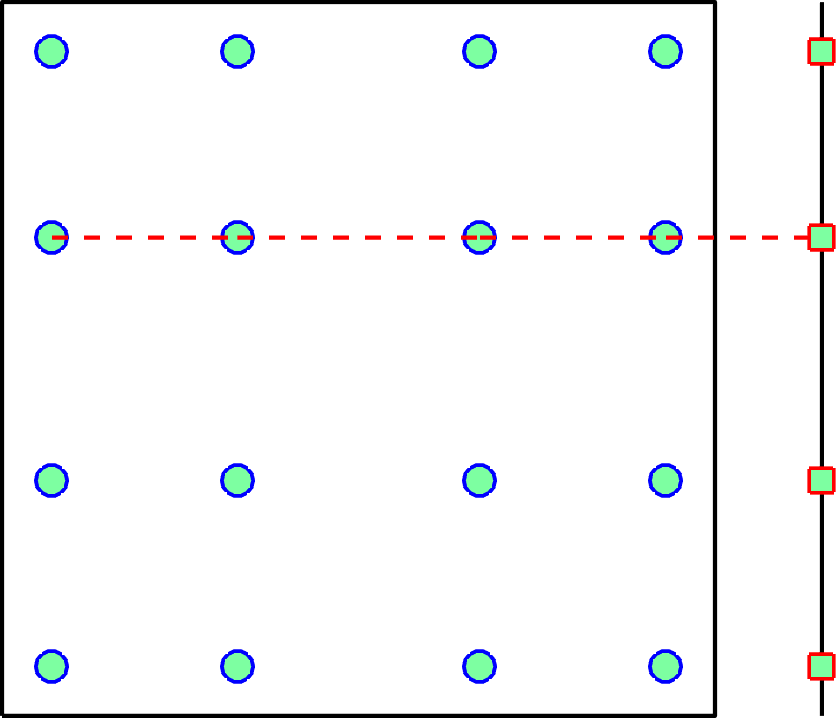
\includegraphics[width=.375\textwidth]{figs/aligned.png}}\label{subfig:aligned}}
\hspace{4em}
\subfloat[Dyadic flux evaluations (composite surface nodes)]{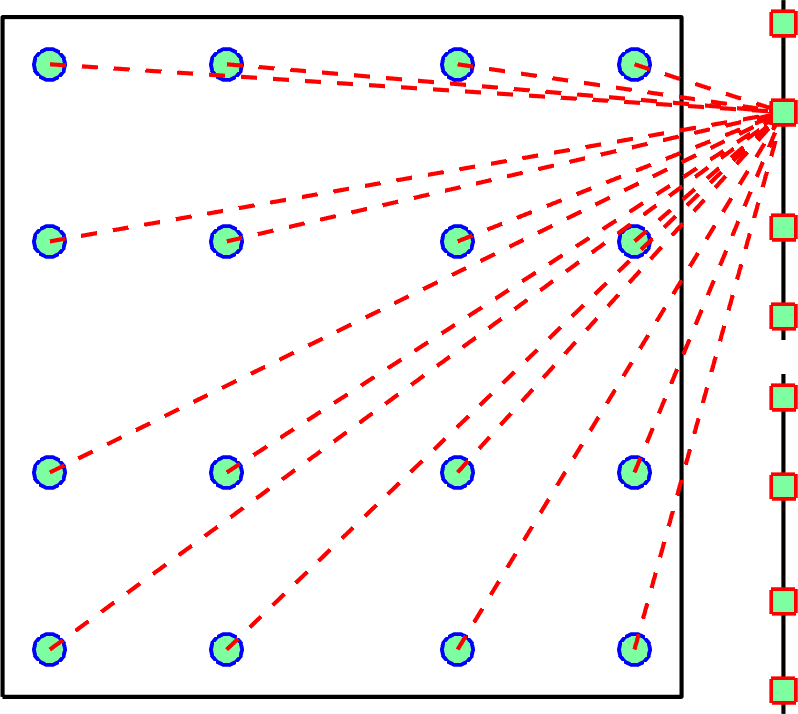
\includegraphics[width=.374\textwidth]{figs/nonaligned.png}\label{subfig:nonaligned}}
\caption{Figure~\ref{subfig:aligned} and \ref{subfig:nonaligned} illustrate when dyadic flux evaluations $\bm{f}^i_S\LRp{\tilde{\bm{u}}_j,\tilde{\bm{u}}_k}$ between nodes are necessary (indicated by dashed red lines) for conforming interfaces (Figure~\ref{subfig:aligned}) and non-conforming interfaces (Figure~\ref{subfig:nonaligned}) under a Gauss collocation scheme.  Conforming interfaces (aligned surface nodes) require evaluations between a surface node and a line of volume nodes, while non-conforming interfaces (nonaligned composite surface nodes) require flux evaluations between a surface node and \textit{all} volume nodes.  The proposed mortar approach (Figure~\ref{subfig:mortar}) reduces the number of dyadic flux evaluations by introducing composite nodes as mortars which couple only to surface nodes. }
\label{fig:fluxsparsity}
\end{figure}


\section{Mortar methods for hybrid and non-conforming meshes}

This work is motivated by complications which arise when designing entropy stable couplings between elements which do not share the same boundary nodes.  This can arise, for example, for hybrid and non-conforming meshes.  

\paragraph{Hybrid meshes:} entropy stable DG methods on hybrid meshes were introduced in \cite{chan2019skew} using a skew-symmetric formulation.  The resulting methods are stable for more arbitrary choices of surface quadrature, in particular when an SBP property may not hold.  

\paragraph{Non-conforming meshes}

On conforming meshes, it is most efficient to utilize both Gauss quadrature for volume integrals and Gauss quadrature for face or surface integrals.  For solutions represented in terms of their values at tensor product volume Gauss nodes, extrapolation to face Gauss nodes can be done in an efficient line-by-line manner using one-dimensional interpolation matrices.  

For non-conforming meshes, it can be advantageous to use composite Gauss quadratures on non-conforming interfaces \cite{Kozdon2018}.  However, interpolating the solution at volume Gauss nodes to split-side Gauss nodes is no longer a one-dimensional operation.  

\section{Mortar formulation}

\begin{figure}[!h]
\centering
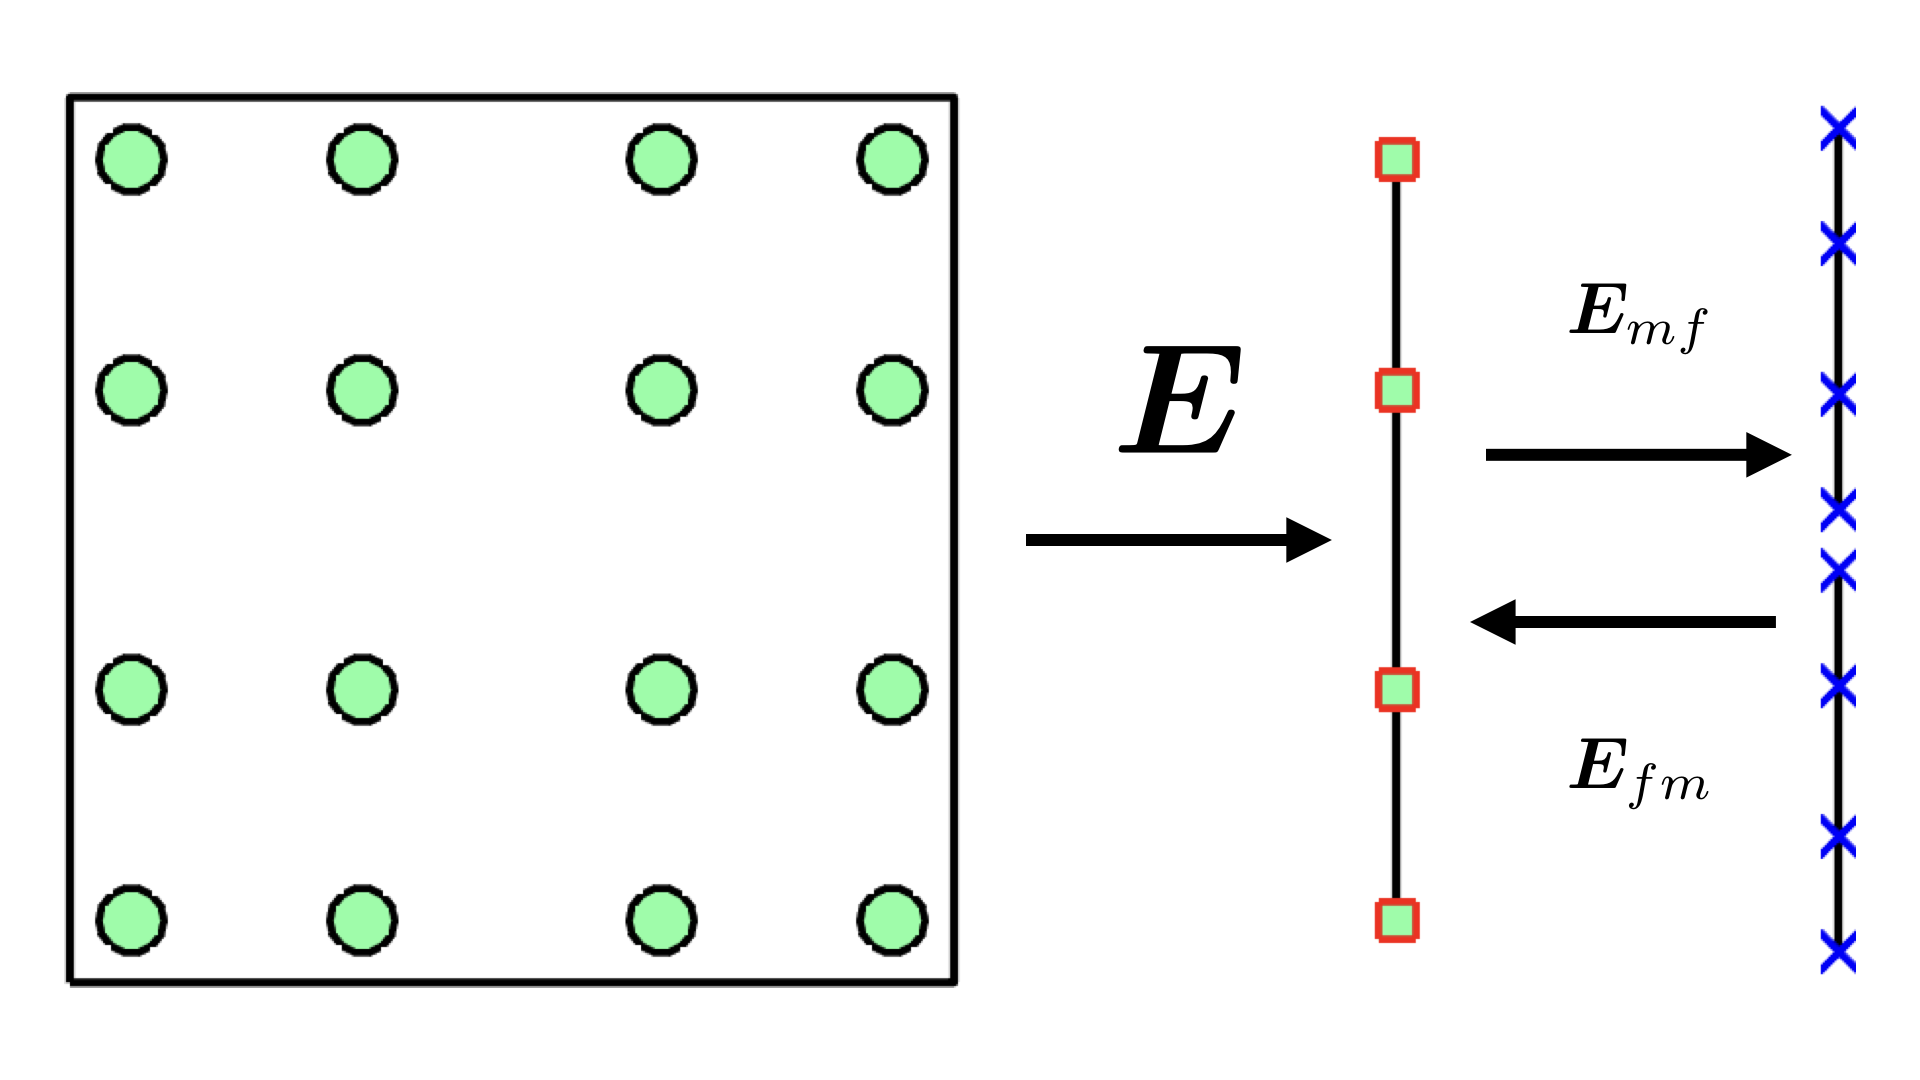
\includegraphics[width=.5\textwidth]{figs/mortar.png}
\caption{Illustration of mortar operators for a Gauss collocation scheme.  The matrix $\bm{E}$ maps from volume quadrature points to surface quadrature points, $\bm{E}_m$ maps from surface to mortar surface points, and $\tilde{\bm{E}}_m$ maps from mortar surface points to surface points. }
\label{fig:gqcon_noncon}
\end{figure}

Let $\bm{V}_q$ and $\bm{V}_f$ denote interpolation matrices which evaluate at volume and surface quadrature points, respectively, and let $\bm{W}, \bm{W}_f$ denote diagonal matrices whose entries consist of volume and surface quadrature weights
\[
\text{\note{add defs of matrices}}
\]

Let $\bm{E} = \bm{V}_f\bm{P}_q$ denote the polynomial mapping which extrapolates values from volume quadrature points to values at surface quadrature points.  We also define $\bm{B}_i$ as the diagonal matrix containing products of quadrature weights and the $i$th component of the outward normal vector $\hat{\bm{n}}_i$
\[
\bm{B}_i = \bm{W}_f \diag{\hat{\bm{n}}_i}.
\]

An entropy stable skew-symmetric formulation can be given on the reference element $\hat{D}$ as follows:
\[
\bm{M}\td{\bm{u}_N}{t} + \begin{bmatrix} \bm{V}_q \\ \bm{V}_f \end{bmatrix}^T
\LRp{\begin{bmatrix}
\bm{Q}_i-\bm{Q}_i^T & \bm{E}^T\bm{B}_i\\
-\bm{B}_i\bm{E} & \bm{0}
\end{bmatrix} \circ \bm{F}_S}\bm{1} + \bm{V}_f^T\bm{B}_i\bm{f}_i^* = 0.  
\]

We incorporate mortars by modifying this formulation.  Let $\bm{V}_m$ denote the matrix which maps volume quadrature points to values at surface \textit{mortar} points.  We also need to introduce interpolation operators $\bm{T}_f, \bm{T}_m$ for surface trace spaces.  Here, $\bm{T}_f$ maps from polynomials on the surface $\partial \hat{D}$ to surface quadrature points, while $\bm{T}_m$ maps from polynomials on $\partial \hat{D}$ to mortar quadrature points.  We can then define surface and mortar mass and projection matrices
\begin{align*}
\bm{M}_m = \bm{T}_m^T\bm{W}_m\bm{T}_m, \qquad \bm{P}_m = \bm{M}_m^{-1}\bm{T}_m^T\bm{W}_m\\
\bm{M}_f = \bm{T}_f^T\bm{W}_f\bm{T}_f, \qquad \bm{P}_f = \bm{M}_m^{-1}\bm{T}_f^T\bm{W}_f.
\end{align*}
Note that we have used the mortar mass matrix $\bm{M}_m$ in the above definition of the face projection.  %This is only necessary if the surface and mortar quadratures do not exactly integrate degree $2N$ polynomials.  If both the surface and mortar quadratures are exact for polynomials of degree $2N$, then $\bm{M}_m = \bm{M}_f$, and no distinction is necessary between the two mass matrices.  

\begin{remark}
In order to show stability, we require that both $\bm{P}_f$ and $\bm{P}_m$ are defined using the same mass matrix.  We have used the mortar mass matrix $\bm{M}_m$ here; however, we could also use the surface mass matrix $\bm{M}_f$ in both $\bm{P}_f$ and $\bm{P}_m$.  We use the mortar mass matrix in this work, as the mortar quadrature is generally more accurate than the surface quadrature for our use cases (e.g.\ hybrid and non-conforming meshes).  
\end{remark}


We can now define operators which map between surface and mortar quadrature points.  Let $\bm{E}_m$ denote the map from surface to mortar points, and let $\tilde{\bm{E}}_m $ denote the map from mortar to surface points.  Both operators are defined through an $L^2$ projection to the trace space and interpolation to appropriate points
\[
\bm{E}_m = \bm{T}_m \bm{P}_f, \qquad \tilde{\bm{E}}_m = \bm{T}_f \bm{P}_m.
\]  
We also define a mortar boundary matrix
\[
\tilde{\bm{B}}_i = \bm{W}_m\diag{\hat{\bm{n}}_i}.
\]
Then, a mortar-based formulation can be given as follows:
\begin{equation}
\bm{M}\td{\bm{u}_N}{t} + \begin{bmatrix} \bm{V}_q \\ \bm{V}_f \\ \bm{V}_m \end{bmatrix}^T
\LRp{\begin{bmatrix}
\bm{Q}_i-\bm{Q}_i^T & \bm{E}^T\bm{B}_i &\\
-\bm{B}_i\bm{E} &  & \bm{B}_i\tilde{\bm{E}}_m \\
& -\tilde{\bm{B}}_i{\bm{E}}_m & 
\end{bmatrix} \circ \bm{F}_S}\bm{1} + \bm{V}_m^T\tilde{\bm{B}}_i\bm{f}_i^* = 0.  
\label{eq:mortar}
\end{equation}
Here, we have appended an extra row and column to the decoupled SBP matrix, and the inter-element numerical flux $\bm{f}^*$ is now computed in terms of the \emph{mortar} nodes.  

We first note that
\begin{align*}
\bm{B}_i\tilde{\bm{E}}_m &= \diag{\bm{W}_f} \bm{T}_f \bm{P}_m = \diag{\hat{\bm{n}}} \bm{W}_f \bm{T}_f \bm{M}_m^{-1}\bm{T}_m\bm{W}_m\\
&=  \bm{W}_f \bm{T}_f \bm{M}_m^{-1}\bm{T}^T_m\bm{W}_m\diag{\hat{\bm{n}}_i} = \bm{P}_f^T\bm{T}^T_m \tilde{\bm{B}}_i = \LRp{\tilde{\bm{B}}_i{\bm{E}}_m}^T
\end{align*}
where we have used that $\bm{W}_m$ is diagonal and that the outward normal $\hat{\bm{n}}_i$ on the reference element is constant over each face.  This implies skew-symmetry of the decoupled SBP operator and entropy stability of the overall system.    


\note{Finish}

\section{A mortar-based implementation}

While the formulation presented above is convenient for analysis, it is computationally expensive to implement.  However, using properties of the mortar matrices $\bm{E}_m, \tilde{\bm{E}}_m$, we can rewrite the above formulation in a way which reflects a traditional mortar-based finite element implementation.  In other words, we wish to implement (\ref{eq:mortar}) such that the only modification from the implementations in \cite{chan2017discretely} is an intermediate step on mortar faces.  

We first note that, since $\bm{E}_m$ maps from surface nodes to mortar nodes, $\bm{V}_m = \bm{E}_m \bm{V}_f$.  Thus, we can rewrite the numerical flux contribution as
\begin{align*}
 \bm{V}_m^T\tilde{\bm{B}}_i\bm{f}_i^* &= \bm{V}_f^T \bm{E}_m^T \bm{W}_m\diag{\hat{\bm{n}}_i} \bm{f}_i^* = \bm{V}_f^T  \bm{P}_f^T\bm{T}_m^T\bm{W}_m\diag{\hat{\bm{n}}_i} \bm{f}_i^*\\
 &= \bm{V}_f^T \bm{W}_f \diag{\hat{\bm{n}}_i} \bm{T}_m\bm{M}_m^{-1}\bm{T}_m^T\bm{W}_m \bm{f}_i^* =  \bm{V}_f^T \bm{B}_i \tilde{\bm{E}}_m\bm{f}_i^*.
\end{align*}

We can similarly reformulate the remaining mortar contributions within (\ref{eq:mortar}).  We decompose $\bm{F}_S$ into interactions between volume nodes, surface nodes, and mortar nodes
\[
\bm{F}_S = \begin{bmatrix}
\bm{F}_S^{vv} & \bm{F}_S^{vs} & \bm{F}_S^{vm}\\
\bm{F}_S^{sv} & \bm{F}_S^{ss} & \bm{F}_S^{sm}\\
\bm{F}_S^{mv} & \bm{F}_S^{ms} & \bm{F}_S^{mm}
\end{bmatrix}
\]
Then, the on-element contributions to (\ref{eq:mortar}) can be expanded as follows
\begin{align*}
&\begin{bmatrix} \bm{V}_q \\ \bm{V}_f \\ \bm{V}_m \end{bmatrix}^T
\LRp{\begin{bmatrix}
\bm{Q}_i-\bm{Q}_i^T & \bm{E}^T\bm{B}_i &\\
-\bm{B}_i\bm{E} &  & \bm{B}_i\tilde{\bm{E}}_m \\
& -\tilde{\bm{B}}_i{\bm{E}}_m & 
\end{bmatrix} \circ \bm{F}_S}\bm{1} \\
&= 
\begin{bmatrix} \bm{V}_q \\ \bm{V}_f \end{bmatrix}^T
\LRp{\begin{bmatrix}
\bm{Q}_i-\bm{Q}_i^T & \bm{E}^T\bm{B}_i\\
-\bm{B}_i\bm{E} & \\
\end{bmatrix} \circ \bm{F}_S}\bm{1} \\
&+ \bm{V}_f^T \LRp{\bm{B}_i\tilde{\bm{E}}_m\circ \bm{F}_S^{sm}}\bm{1} - \bm{V}_m^T \LRp{ \tilde{\bm{B}}_i\bm{E}_m \circ \bm{F}_S^{ms}}\bm{1}
\end{align*}
Since multiplication by diagonal matrices $\bm{B}_i, \tilde{\bm{B}}_i$ is associative under the Hadamard product, the latter terms can be rewritten as 
\begin{align*}
 \bm{V}_f^T \LRp{\bm{B}_i\tilde{\bm{E}}_m\circ \bm{F}_S^{sm}}\bm{1} &=  \bm{V}_f^T \bm{B}_i \LRp{\tilde{\bm{E}}_m\circ \bm{F}_S^{sm}}\bm{1}\\
\bm{V}_m^T \LRp{ \tilde{\bm{B}}_i\bm{E}_m \circ \bm{F}_S^{ms}}\bm{1} &= \bm{V}_m^T \tilde{\bm{B}}_i \LRp{ \bm{E}_m \circ \bm{F}_S^{ms}}\bm{1} = \bm{V}_f^T \bm{B}_i \tilde{\bm{E}}_m \LRp{ \bm{E}_m \circ \bm{F}_S^{ms}}\bm{1} 
\end{align*}
Then, (\ref{eq:mortar}) can be rewritten as 
\begin{align}
\bm{M}\td{\bm{u}_N}{t} &+ 
\begin{bmatrix} \bm{V}_q \\ \bm{V}_f \end{bmatrix}^T
\LRp{\begin{bmatrix}
\bm{Q}_i-\bm{Q}_i^T & \bm{E}^T\bm{B}_i\\
-\bm{B}_i\bm{E} & \\
\end{bmatrix} \circ \bm{F}_S}\bm{1} + \bm{V}_f^T\bm{B}_i \tilde{\bm{f}}^*_i = 0 \label{eq:mortar2}\\
\tilde{\bm{f}}^*_i &= \tilde{\bm{E}}_m\bm{f}^*_i + \LRp{\tilde{\bm{E}}_m\circ \bm{F}_S^{sm}}\bm{1} - \tilde{\bm{E}}_m \LRp{ \bm{E}_m \circ \bm{F}_S^{ms}}\bm{1} 
\nonumber
\end{align}
If the surface and mortar nodes are identical, then 
\[
\bm{E}_m = \tilde{\bm{E}}_m = \bm{I}, \qquad \LRp{\tilde{\bm{E}}_m \circ \bm{F}_S^{sm}}\bm{1} = \LRp{ \bm{E}_m \circ \bm{F}_S^{ms}}\bm{1}
\]
and the correction terms within $\tilde{\bm{f}}^*$ cancel out, and we recover the original scheme from \cite{chan2017discretely}.

Note that in (\ref{eq:mortar2}), the only interactions between surface and mortar nodes occurs within the computation of $\tilde{\bm{f}}^*_i$, which can be done solely on mortar interfaces.  The computational structure of 
\begin{enumerate}
\item Compute volume contributions to the RHS
\item Communicate surface contributions to mortar interfaces and compute $\tilde{\bm{f}}^*_i$.
\item Communicate $\tilde{\bm{f}}^*_i$ back to each element.  
\end{enumerate}

\section{Error estimates}

\note{Weak derivative vs strong derivative error estimates.  SBP yields that the skew-symmetric form is equivalent to weak form.}

\note{Line DG approach can work, but it's flipped: we increase quadrature strength in the direction \emph{orthogonal} to derivative instead.  May improve accuracy over GLL by giving equivalence w/skew form.}

\section{Numerical experiments}

Figure~\ref{subfig:noncon} shows preliminary results for the 2D compressible Euler equations by the PI on a manually constructed non-conforming quadrilateral mesh, with volume, surface, and mortar quadratures constructed from one-dimensional GLL or Gauss quadrature rules.  The PI has verified that this preliminary implementation of the mortar-based formulation is discretely entropy stable.  A preliminary accuracy analysis for the skew-symmetric formulation (\ref{eq:esdgSkew}) also suggests that GLL quadrature should achieve an $O(h^N)$ rate of convergence and that Gauss quadrature should achieve an $O(h^{N+1})$ rate of convergence.  Both predicted rates are confirmed in Figure~\ref{subfig:noncon}.

\begin{figure}
\centering
\subfloat[Coarse non-conforming mesh]{\raisebox{3em}{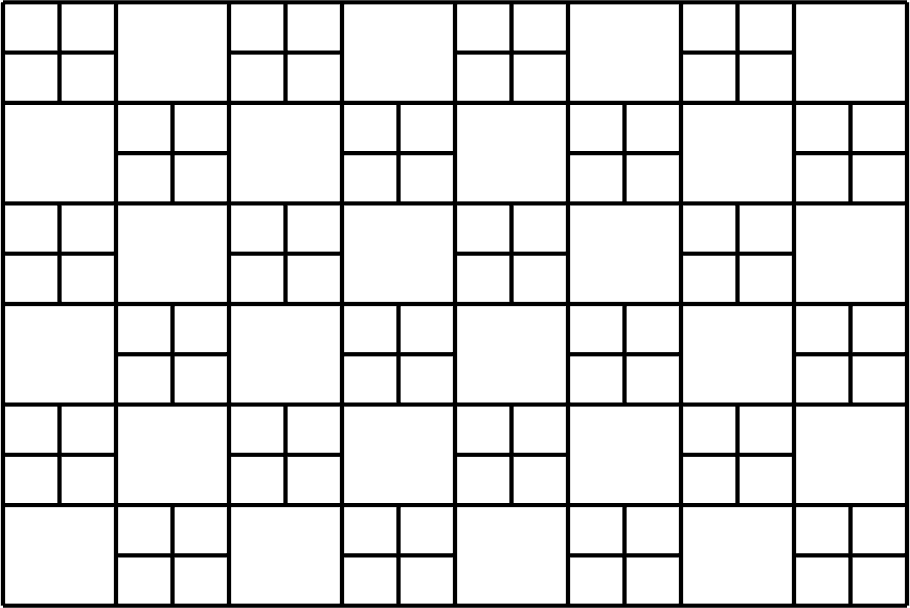
\includegraphics[width=.425\textwidth]{figs/noncon_mesh.png}}}
\hspace{.25em}
\subfloat[Sub-optimal rates if under-integrated]{
\begin{tikzpicture}
\begin{loglogaxis}[
    width=.5\textwidth,
    xlabel={Mesh size $h$},
    ylabel={$L^2$ errors}, 
    xmax=1,
    ymin=5e-5, ymax=5,
    legend pos=south east, legend cell align=left, legend style={font=\tiny},	
    xmajorgrids=true, ymajorgrids=true, grid style=dashed,
    legend entries={Lobatto, Gauss, Lobatto-Gauss}    
]
\pgfplotsset{
cycle list={{blue, mark=*}, {red, dashed ,mark=square*},{black, dashdotted ,mark=triangle*}}
}
% N = 1
\addplot+[semithick, mark options={solid, fill=markercolor}]
coordinates{(0.333333,2.6993)(0.166667,1.6718)(0.0833333,0.7792)(0.0416667,0.29211)};
\addplot+[semithick, mark options={solid, fill=markercolor}]
coordinates{(0.333333,2.0534)(0.166667,0.7966)(0.0833333,0.2022)(0.0416667,0.0449413)};
\addplot+[semithick, mark options={solid, fill=markercolor}]
coordinates{(0.333333,2.94072)(0.166667,1.73057)(0.0833333,0.97069)(0.0416667,0.487387)};

% N = 2
\addplot+[semithick, mark options={solid, fill=markercolor}]
coordinates{(0.333333,1.1609)(0.166667,0.3562)(0.0833333,0.0768)(0.0416667,0.0192197)};
\addplot+[semithick, mark options={solid, fill=markercolor}]
coordinates{(0.333333,0.7191)(0.166667,0.141)(0.0833333,0.0178)(0.0416667,0.00243087)};
\addplot+[semithick, mark options={solid, fill=markercolor}]
coordinates{(0.333333,1.20291)(0.166667,0.347365)(0.0833333,0.0606688)(0.0416667,0.0144843)};

% N = 3
\addplot+[semithick, mark options={solid, fill=markercolor}]
coordinates{(0.333333,0.551145)(0.166667,0.0754237)(0.0833333,0.0100808)(0.0416667,0.00120633)};
\addplot+[semithick, mark options={solid, fill=markercolor}]
coordinates{(0.333333,0.352706)(0.166667,0.0258415)(0.0833333,0.00211953)(0.0416667,0.000132969)};
\addplot+[semithick, mark options={solid, fill=markercolor}]
coordinates{(0.333333,0.557084)(0.166667,0.0671373)(0.0833333,0.00744086)(0.0416667,0.000837905)};

% N = 4
\addplot+[semithick, mark options={solid, fill=markercolor}]
coordinates{(0.333333,0.267668)(0.166667,0.0192603)(0.0833333,0.00140341)};
\addplot+[semithick, mark options={solid, fill=markercolor}]
coordinates{(0.333333,0.128217)(0.166667,0.00779943)(0.0833333,0.000270803)};
\addplot+[semithick, mark options={solid, fill=markercolor}]
coordinates{(0.333333,0.212176)(0.166667,0.0151178)(0.0833333,0.000826307)};

\node at (axis cs:.55,2.5) {$N = 1$};
\node at (axis cs:.55,1.0) {$N = 2$};
\node at (axis cs:.55,.42) {$N = 3$};
\node at (axis cs:.55,.16) {$N = 4$};
\end{loglogaxis}
\end{tikzpicture}
}
\caption{Blah}
\end{figure}

\subsection{Gauss Lobatto quadrature}

\subsection{Gauss quadrature}

\bibliographystyle{unsrt}
\bibliography{dg}


\end{document}


